\documentclass{report}
\usepackage{graphicx}
\usepackage[fleqn]{amsmath}
\usepackage[utf8]{inputenc}
\usepackage[fontsize=15pt]{fontsize}
\usepackage{ragged2e}
\usepackage{blindtext}


\title{\textbf{ME5010 : Logistic Map}}
\usepackage{geometry}
 \geometry{
 a4paper,
 total={170mm,257mm},
 left=20mm,
 top=20mm,
 }
\begin{document}
\author{Shyam Sridhar\\ Nitesh Singh \\ Rudramuni TS \\ Pavan Kumar \\ Aman Gautam }
\maketitle

\section{Introduction}
\raggedright

\begin{center}$x_{n+1} = rx_n(1-x_n)$\end{center}
Logistic Equation is primarily know for modeling population growth of animals and it is part \textbf{Chaos Theory}, which is branch of mathematics that demonstrates how deterministic mathematical system could lead to unpredictability.

Logistic equation is characterized by it's sensitivity to input parameters. Very small changes in $x_0$ and $r$ could lead to drastic changes in predictions, and thus leading to Chaos. Due to this particular nature logistic map was once used to generate array of seemingly unrelated numbers also called pseudo-random number. It could generate unpredictability from deterministic machine. Beside that it is also used in cryptography for encryption of data where encrypted data would be very sensitive to the key i.e small variation in key would not decrypt/decode the encrypted data allowing only one and one unique key to decrypt the data.

In this project our aim is to explore behaviour of logistic map. It's sensitivity to initial parameters, period doubling, unpredictability and device a pseudo-random number generator (PRNG). We will use same PRNG to encrypt an image.

\section{Uniformity in Randomness}
\raggedright

Reason why I use \textbf{pseudo}-random numbers because for exactly same starting conditions or initial values we will have same array of numbers that are deterministic. As a matter of fact even pre-built random number generator in python also gives same array of numbers if we query random numbers with a particular seed or initial parameter.

The idea behind generating pseudo-random numbers from such system is their sensitivity  to initial conditions itself. Even change in orders of $10^{-6}$ would generate an entirely different array of numbers. Determining the seed or initial condition is not straight-forward given a state of certain point in future. Moreover, explaining systems that are hypersensitive to initial parameters is forte of Chaos Theory

\begin{quote}
When a butter fly flutters it's wings in one part of the world, it can eventually cause a hurricane in another.  (Edward Norton Lorenz)
\end{quote}


\newpage
\section{Logistic Equation}
\raggedright
The following equation also called logistic equation is used to model population growth.
\begin{equation}
x_{n+1} = rx_n(1-x_n) \nonumber
\end{equation}
where:

$x_n$ = population in $n$th generation,

$r$ = growth rate

\begin{figure}[!h]
    \centering
    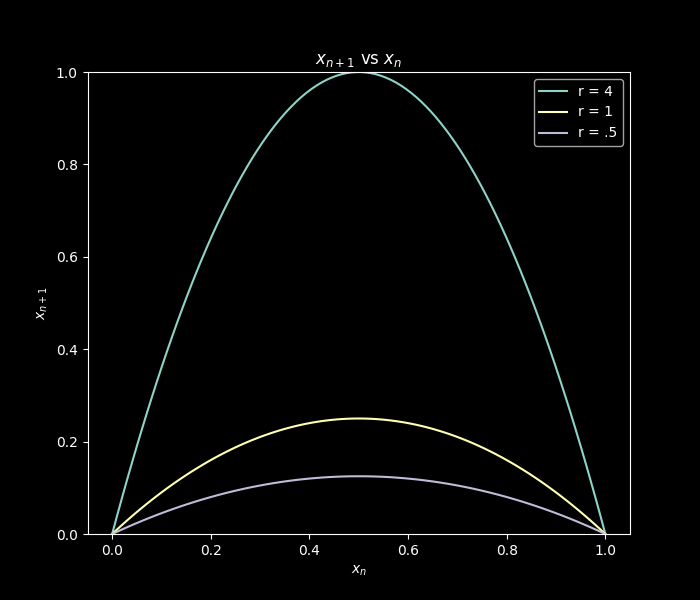
\includegraphics[scale=.5]{images/xnvsnp1.png}
    \caption{$x_{n+1}$ vs $x_n$ (Such functions are also called single humped functions)}
    \label{fig:my_label}
\end{figure}

For $r \in [0, 4]$ the function $x_{n+1}$ maps the closed interval [0, 1] into itself. We shall
restrict our attention to these values of r. Also we'll see r is the main factor contributing to unpredictability of equation.

As observed from the graph below $x_{n}$ is not exactly predictable for every r.

\begin{figure}[!h]
    \centering
    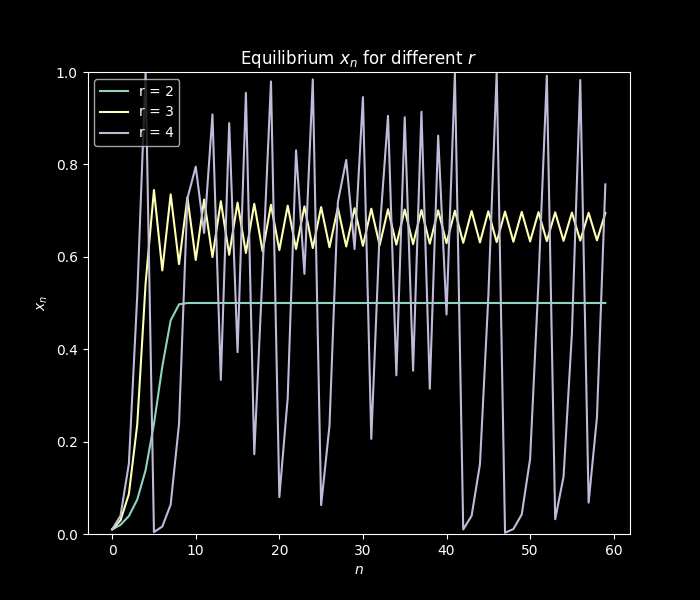
\includegraphics[scale=.4]{images/eqfordifr.png}
    \caption{$x_n$ at equilibrium for different r's}
    \label{fig:my_label2}
\end{figure}

On varying r and plotting equilibrium $x_{n}$ we get the following observations.

\begin{itemize}
  \item $r < 3$ One Equilibrium position of x is seen.
  \item $r > 3$ Two Equilibrium position of x is seen.
  \item As r is increased further we have multiple equilibrium positions
\end{itemize}
\newpage
\subsection{Fixed Points}

\raggedright

Equation can be said to be converging when. $x_{n+1} \to x_n$

Thus, we can write
\begin{equation}
    x = rx(1-x) \nonumber
\end{equation}

From above equation we get the following solutions or equilibrium points.\\

$x = 0$ and $x = 1 - \frac{1}{r}$
\begin{itemize}
  \item For $r \in [0,1)$ $x = 0$ acts as attractor (solution converges to this point)
  \item For $r = 1$, $x = 0$ acts as repellor (x seems to diverge from x = 0 line)
  \item And $x = 1 - \frac{1}{r}$ is an attractor for $r \in (1,3)$ and a repeller for $r > 3$.
\end{itemize}


This can be obtained from the slope of $f_r = rx(1-x)$ at x, \newline


that is equal to $r(1-2x)$ for points 0 and $1-\frac{1}{r}$.\newline

$f'_r(0) = r$  and $f'_r(1-\frac{1}{r}) = 2-r$\newline

Absolute value of Slope less than 1 implies $x_n$ will be attracted to the solution and vica-versa. Observe there is no single point attractors for $r>3$ thus explaining why there is no single solution in that case.

In fact, as r continues to increase after 3, $x_n$ converges to a permanent oscillation between two values depending on r. Increasing r further it starts oscillating between 4 values and so-on. This brings us to our next topic of \textbf{period-doubling} observed in logistic equation. This also connects logistic equation with mathematical fractals.
\newpage
\subsection{Period Doubling}
\raggedright
In this section we will see why actually solution starts oscillating between multiple points and doubles with r.
\begin{equation}
    f_r = rx(1-x) \nonumber
\end{equation}
\begin{equation}
    fof_r = rf_r(1-f_r) \nonumber
\end{equation}

For convergence, we will try to find solution of the following equation.
\begin{equation}
     fof_r = x \nonumber
\end{equation}
\begin{equation}
    x(r^2x^2 - (r^2+r)x+(1+r)) = 0 \nonumber
\end{equation}

Solving and simplifying this equation we get three solution 0 and other two solutions are roots of the following equation, \newline
\begin{equation}
r^2x^2 - (r^2+r)x+(1+r) = 0 \nonumber
\end{equation}
\begin{equation}
x^2 - (1+\frac{1}{r})x + \frac{1}{r^2} + \frac{1}{r} = 0
\end{equation}


If $q_1$ and $q_2$ are solutions of the above equation then they can be real if

\begin{equation}
    (\frac{r+1}{r}) \geq \frac{4(1+r)}{r^2} \nonumber
\end{equation}


This on simplification leading to \newline

$r \geq 3$. This makes sense because cycle of period 2 exist after r = 3 \newline
Again to find where equilibrium is attracted to we will find slope of $f'_r(q_1)f'_r(q_2)$ and find values of r for which it's slope $\in [-1,1]$ where $f'_r = r(1-2x)$

\begin{align}
f'_r(q_1)f'_r(q_2) &= r^2(1 - 2q_1)(1 - 2q_2) \nonumber \\
 &= r^2(1 - 2(q_1+q_2) + 4q_1q_2) \nonumber
\end{align}

Using (1) in this equation

\begin{equation}
f'_r(q_1)f'_r(q_2) = -r^2 + 2r + 4
\end{equation}

\newpage

Equation (2) is 1 when $r = 3$, and for $r > 3$  it decreases and reaches value of -1 when $r = 1 + \sqrt[]{6} = 3.449..$
\newline

Thus this shows that solution will oscillate between two points $q_1$ and $q_2$ for values of $r \in (3,3.449..)$

Like this at certain r's we will get period doubling first three are,
\begin{align}
    r_0 &= 1 \nonumber \\
    r_1 &= 3 \nonumber \\
    r_2 &= 1 + \sqrt[]{6} \nonumber \\
    r_3 &= 3.544... \nonumber
\end{align}
This is also called cascade of period doubling, Note  $r_3$ is not evaluated in above calculation I took it from graph I made

Let us define a term which looks like
\begin{equation}
    \delta_k = \frac{r_k - r_{k-1}}{r_{k+1} - r_k}
\end{equation}

For $k = 1$, $\delta_1 \approx 4.44949$ \newline

Graphically we will see this value approaches to \textbf{4.669202...} . This is an universal constant like $\pi$ know as \textbf{feigenbaun's ratio}. It appears in many chaotic system like dripping faucet, firing of neurons in brain, fluid behaviour and is exactly the same.
It is also observed at $r = 3.829$ the equilibrium oscillates in period of 3 because $fofof_r = x$ have three roots. \newline

\begin{figure}[!h]
    \centering
    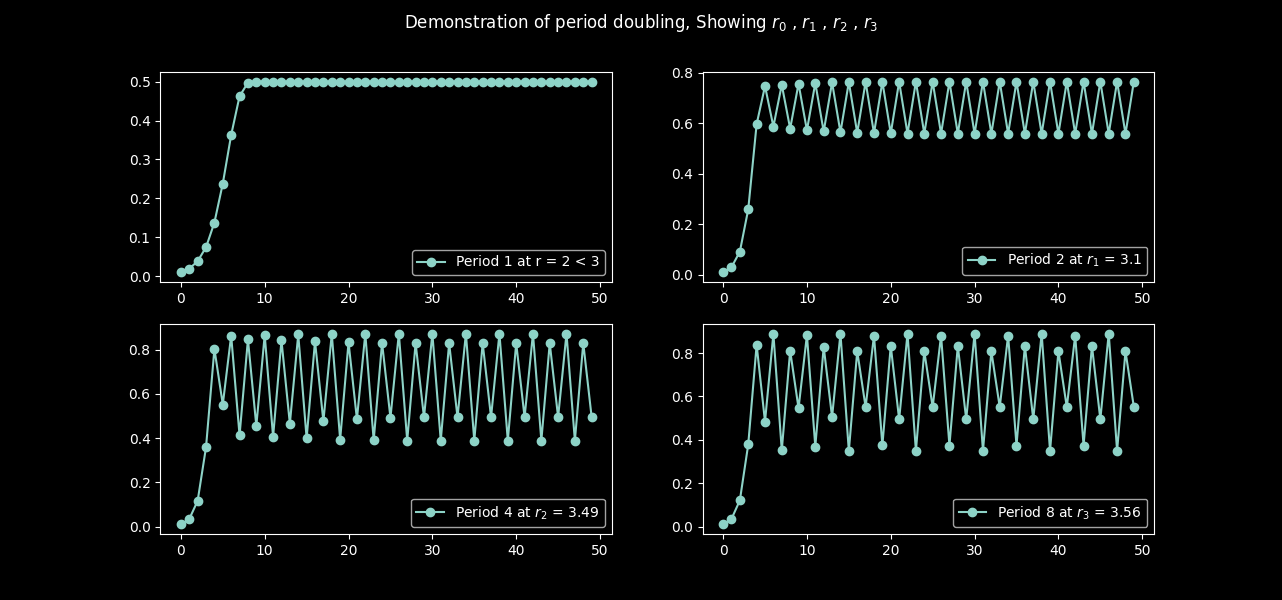
\includegraphics[scale=.45]{images/period2ing.png}
    \caption{Demonstrating period doubling with progression of r}
    \label{fig:my_label3}
\end{figure}

\subsection{Bifurcation Map}
\raggedright
A Bifurcation Diagram is a visual summary of the succession of period-doubling produced as r increases\footnote[1]{https://www.vanderbilt.edu/AnS/psychology/cogsci/chaos/workshop/BD.html}.

In our logistic equation \textbf{r} is the bifurcation parameter and it's show on horizontal axis. The bifurcation diagram shows the forking of the periods of stable orbits from 1 to 2 to 4 to 8 etc. Each of these bifurcation points is a period-doubling bifurcation. The ratio of the lengths of successive intervals between values of r for which bifurcation occurs converges to the first Feigenbaum constant.\footnote[2]{https://en.wikipedia.org/wiki/Bifurcation\_diagram}

\begin{figure}[!h]
    \centering
    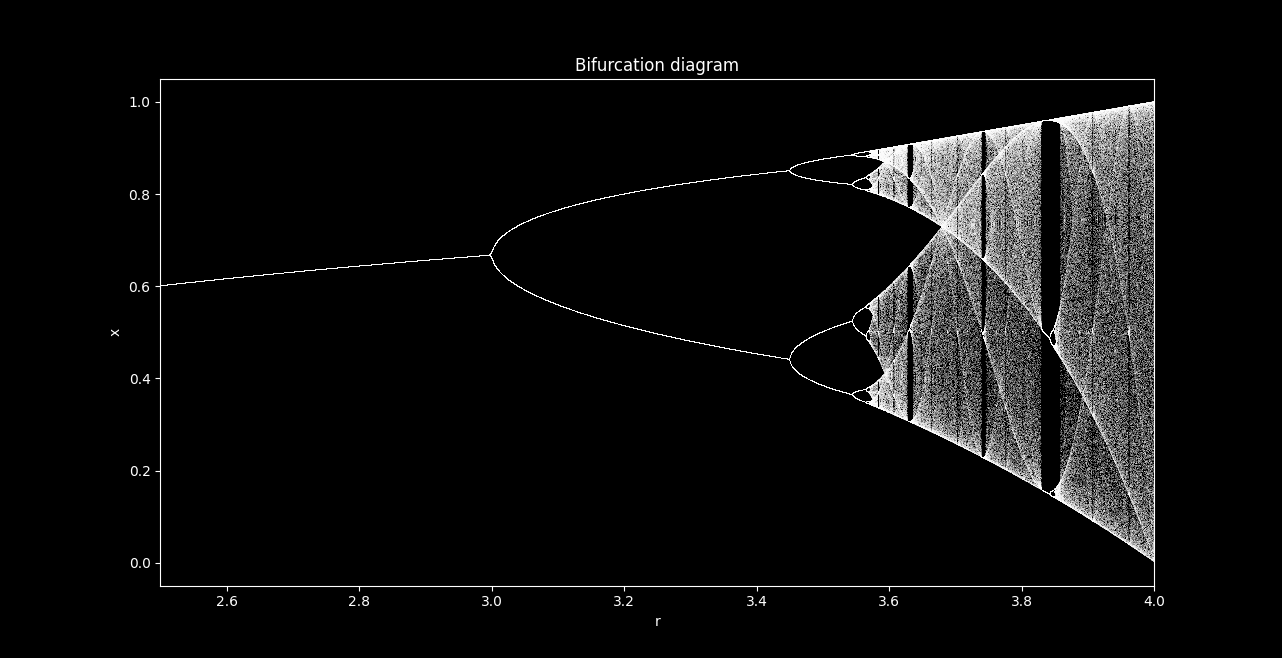
\includegraphics[scale=.45]{images/BifurcationDiag.png}
    \caption{Bifurcation Diagram for $r \in [2.5,4]$}
    \label{fig:my_label4}
\end{figure}

\end{document}

